\section{Цель работы}

\begin{enumerate}
    \item Измерение зависимости магнитной индукции в ферромагнетике от напряженности магнитного поля $B = B(H)$
    
    \item Определение по предельной петле гистерезиса индукции насыщения, остаточной индукции и коэрцитивной силы
    
    \item Получение зависимости магнитной проницаемости от напряженности магнитного поля $\mu = \mu(H)$ и оценка максимального значения величины магнитной проницаемости
    
    \item Расчет мощности потерь энергии в ферромагнетике в процессе его перемагничивания
\end{enumerate}

\section{Задачи, решаемые при выполнении работы}

\begin{enumerate}
    \item Измерение зависимости магнитной индукции в ферромагнетике от напряженности магнитного поля $B = B(H)$
    
    \item Определение по предельной петле гистерезиса индукции насыщения, остаточной индукции и коэрцитивной силы
    
    \item Получение зависимости магнитной проницаемости от напряженности магнитного поля $\mu = \mu(H)$ и оценка максимального значения величины магнитной проницаемости
    
    \item Расчет мощности потерь энергии в ферромагнетике в процессе его перемагничивания
\end{enumerate}

\section{Объект исследования}

Ферромагнитный материал (сердечник трансформатора), который имеет прямоугольную форму с прямоугольным поперечным сечением. 

\section{Метод экспериментального исследования}

Многократные измерения с использованием метода осциллографических изображений. 
Метод основан на визуализации петли гистерезиса на экране цифрового запоминающего осциллографа (ЦЗО) 
и последующем расчете магнитных характеристик по параметрам осциллограммы.

\section{Измерительные приборы}

\begin{table}[h]
\centering
\caption{Список измерительных приборов}
\begin{tabular}{|l|l|p{5cm}|p{5cm}|}
\hline
\textbf{Прибор} & \textbf{Модель} \\
\hline
Цифровой запоминающий осциллограф & GDS-71102B \\
\hline
Генератор сигналов & АКИП-3409/2  \\
\hline
\end{tabular}
\end{table}

\newpage
\section{Схема установки}

\begin{figure}[h]
    \centering
    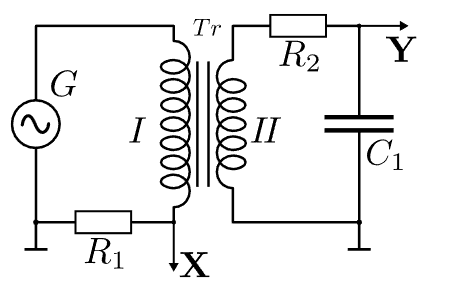
\includegraphics[width=0.5\linewidth]{pic/sp20260416_234252_464.png}
    \caption{Принципиальная электрическая схема установки}
    \label{fig:placeholder}
\end{figure}

\section{Рабочие формулы и исходные данные}

\subsection{Исходные данные}

\begin{center}
\begin{tabular}{|l|c|l|}
\hline
\textbf{Параметр} & \textbf{Обозначение} & \textbf{Значение} \\
\hline
Сопротивление резистора & $R_1$ & $68$~Ом $\pm 10\%$ \\
\hline
Сопротивление резистора & $R_2$ & $470$~кОм $\pm 10\%$ \\
\hline
Емкость конденсатора & $C_1$ & $0{,}47$~мкФ $\pm 10\%$ \\
\hline
Площадь поперечного сечения ферромагнетика & $S$ & $0{,}64 \pm 0{,}05$~см$^2$ \\
\hline
Средняя длина ферромагнетика & $L$ & $7{,}8 \pm 0{,}1$~см \\
\hline
Число витков намагничивающей обмотки & $N_1$ & $1665$~вит \\
\hline
Число витков измерительной обмотки & $N_2$ & $970$~вит \\
\hline
Частота генератора & $f$ & $20$~Гц \\
\hline
Магнитная постоянная & $\mu_0$ & $4\pi \cdot 10^{-7}$~Гн/м \\
\hline
\end{tabular}
\end{center}

\subsection{Рабочие формулы}

Масштабирующие коэффициенты:
\[
\alpha = \frac{N_1}{L R_1}, \qquad 
\beta = \frac{R_2 C_1}{N_2 S}
\]

Расчет напряженности магнитного поля и индукции:
\[
H = \alpha \cdot K_x \cdot x, \qquad B = \beta \cdot K_y \cdot y
\]
где $K_x$, $K_y$ -- цены деления осциллографа по осям (В/дел), $x$, $y$ -- координаты в делениях.

Магнитная проницаемость:
\[
\mu = \frac{B}{\mu_0 H}
\]

Мощность потерь на перемагничивание:
\[
P = \chi \cdot S_{\text{пг}}, \quad \text{где} \quad 
\chi = K_x K_y \frac{N_1 R_2 C_1}{N_2 R_1} f
\]

\section{Результаты прямых измерений и их обработки}

\subsection{Расчет масштабирующих коэффициентов}

На основании исходных данных рассчитаны масштабирующие коэффициенты:

\[
\alpha = \frac{N_1}{L R_1} = \frac{1665}{0{,}078 \cdot 68} \approx 313{,}91 \text{ А/(В}\cdot\text{м)}
\]

\[
\beta = \frac{R_2 C_1}{N_2 S} = \frac{470000 \cdot 0{,}47 \cdot 10^{-6}}{970 \cdot 0{,}64 \cdot 10^{-4}} \approx 3{,}588 \text{ Тл/В}
\]

\subsection{Таблица 1. Определение коэрцитивной силы и остаточной индукции}
Измерены координаты пересечения предельной петли гистерезиса с осями при $U=20$~В, $K_x=20$~мВ/дел, $K_y=10$~мВ/дел.

\[
H_c = \alpha \cdot K_x \cdot X_c = 313{,}91 \cdot 0{,}02 \cdot 2 \approx 12{,}6 \text{ А/м}
\]
\[
B_r = \beta \cdot K_y \cdot Y_r = 3{,}588 \cdot 0{,}01 \cdot 3 \approx 0{,}108 \text{ Тл}
\]

\begin{center}
\begin{tabular}{|c|c|c|c|}
\hline
$X_c$, дел. & $Y_r$, дел. & $H_c$, А/м & $B_r$, Тл \\
\hline
2 & 3 & 12{,}6 & 0{,}108 \\
\hline
\end{tabular}
\end{center}

\subsection{Таблица 2. Определение параметров насыщения}
Координаты вершины петли гистерезиса при $U=20$~В.

\[
H_m = \alpha \cdot K_x \cdot X_m = 313{,}91 \cdot 0{,}02 \cdot 20 = 125{,}6 \text{ А/м}
\]
\[
B_m = \beta \cdot K_y \cdot Y_m = 3{,}588 \cdot 0{,}01 \cdot 10 = 0{,}359 \text{ Тл}
\]
\[
\mu_m = \frac{B_m}{\mu_0 H_m} = \frac{0{,}359}{4\pi \cdot 10^{-7} \cdot 125{,}6} \approx 2274 \text{ Гн/м}
\]

\begin{center}
\begin{tabular}{|c|c|c|c|c|}
\hline
$X_m$, дел. & $Y_m$, дел. & $H_m$, А/м & $B_m$, Тл & $\mu_m$, Гн/м \\
\hline
20 & 10 & 125{,}6 & 0{,}359 & 2274 \\
\hline
\end{tabular}
\end{center}

\subsection{Таблица 3. Зависимость $B(H)$ и $\mu(H)$ при снижении амплитуды}

\textbf{Пример расчета для $U=10$~В:}
\[
H = \alpha \cdot K_x \cdot X = 313{,}91 \cdot 0{,}01 \cdot 13 = 40{,}8 \text{ А/м}
\]
\[
B = \beta \cdot K_y \cdot Y = 3{,}588 \cdot 0{,}005 \cdot 10 = 0{,}179 \text{ Тл}
\]
\[
\mu = \frac{B}{\mu_0 H} = \frac{0{,}179}{4\pi \cdot 10^{-7} \cdot 40{,}8} \approx 3499 \text{ Гн/м}
\]

\begin{center}
\small
\begin{tabular}{|c|c|c|c|c|c|c|c|}
\hline
$U$, В & $X$, дел. & $K_x$, мВ/дел & $H$, А/м & $Y$, дел. & $K_y$, мВ/дел & $B$, Тл & $\mu$, Гн/м \\
\hline
20 & 20 & 20 & 125{,}6 & 10 & 10 & 0{,}359 & 2274 \\
\hline
19 & 19 & 20 & 119{,}3 & 10 & 10 & 0{,}359 & 2394 \\
\hline
18 & 17 & 20 & 106{,}7 & 9 & 10 & 0{,}323 & 2409 \\
\hline
17 & 15 & 20 & 94{,}2 & 9 & 10 & 0{,}323 & 2730 \\
\hline
16 & 13 & 20 & 81{,}6 & 8 & 10 & 0{,}287 & 2801 \\
\hline
15 & 12 & 20 & 75{,}3 & 16 & 5 & 0{,}287 & 3032 \\
\hline
14 & 10 & 20 & 62{,}8 & 15 & 5 & 0{,}269 & 3411 \\
\hline
13 & 18 & 10 & 56{,}5 & 14 & 5 & 0{,}251 & 3546 \\
\hline
12 & 16 & 10 & 50{,}2 & 13 & 5 & 0{,}233 & 3701 \\
\hline
11 & 14 & 10 & 43{,}9 & 11 & 5 & 0{,}197 & 3577 \\
\hline
10 & 13 & 10 & 40{,}8 & 10 & 5 & 0{,}179 & 3499 \\
\hline
9 & 11 & 10 & 34{,}5 & 9 & 5 & 0{,}161 & 3718 \\
\hline
8 & 18 & 5 & 28{,}3 & 8 & 5 & 0{,}144 & 4041 \\
\hline
7 & 15 & 5 & 23{,}5 & 18 & 2 & 0{,}129 & 4358 \\
\hline
6 & 14 & 5 & 22{,}0 & 16 & 2 & 0{,}115 & 4162 \\
\hline
5 & 12 & 5 & 18{,}8 & 14 & 2 & 0{,}100 & 4250 \\
\hline
\end{tabular}
\normalsize
\end{center}

\textbf{Анализ:} 
Максимальная магнитная проницаемость $\mu_{\max} \approx 4358$~Гн/м достигается при $U = 7$~В 
, напряженность поля $H \approx 23{,}5$~А/м.

\subsection{Расчет мощности потерь}

По осциллограмме предельной петли гистерезиса (при $U=20$~В) определена площадь $S_{\text{пг}} \approx 8$~клеток.

Коэффициент $\chi$ (при $K_x = 0{,}02$~В, $K_y = 0{,}01$~В, $f = 20$~Гц):
\[
\chi = K_x K_y \frac{N_1 R_2 C_1}{N_2 R_1} f = 0{,}02 \cdot 0{,}01 \cdot \frac{1665 \cdot 470000 \cdot 0{,}47 \cdot 10^{-6}}{970 \cdot 68} \cdot 20 \approx 5{,}57 \cdot 10^{-4}
\]

Мощность потерь:
\[
P = \chi \cdot S_{\text{пг}} \approx 5{,}57 \cdot 10^{-4} \cdot 8 \approx 4{,}5 \cdot 10^{-3} \text{ Вт} \approx 4{,}5 \text{ мВт}
\]

\textbf{Оценка погрешности:}
\[
\varepsilon_P = \sqrt{\left(\frac{\Delta K_x}{K_x}\right)^2 + \left(\frac{\Delta K_y}{K_y}\right)^2 + \left(\frac{\Delta R_2}{R_2}\right)^2 + \left(\frac{\Delta C_1}{C_1}\right)^2 + \left(\frac{\Delta S_{\text{пг}}}{S_{\text{пг}}}\right)^2} \approx 20\%
\]

\textbf{Итоговый результат:}
\[
P = (4{,}5 \pm 0{,}9) \text{ мВт}
\]

\newpage

\section{Графики}

\begin{figure}[h]
    \centering
    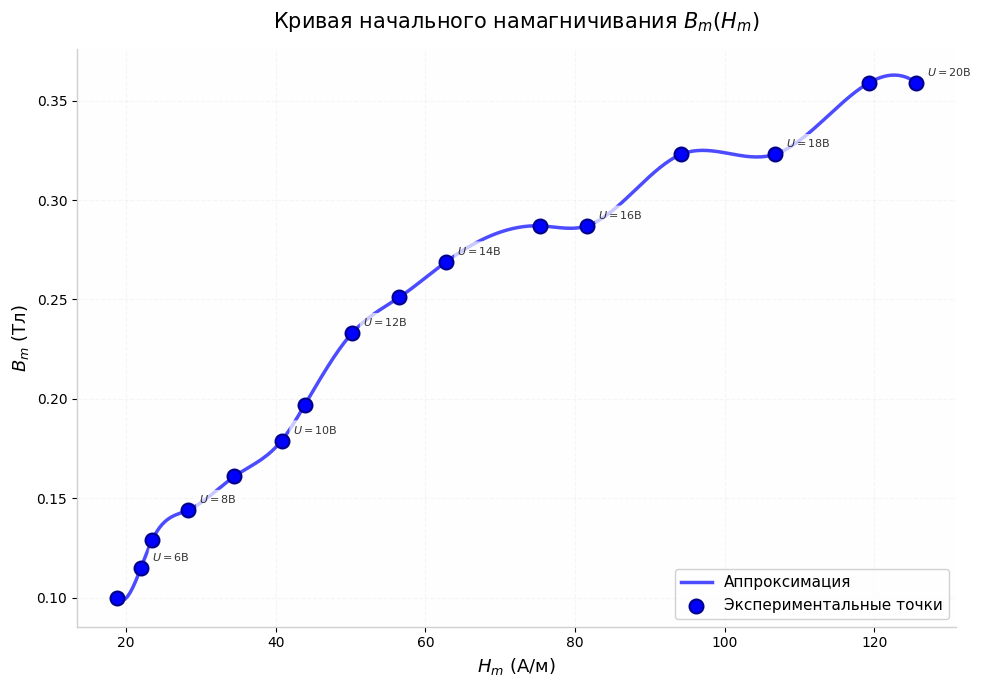
\includegraphics[width=0.5\linewidth]{pic/image.png}
    \caption{Кривая начального намагничивания $B_m(H_m)$}
    \label{fig:placeholder}
\end{figure}

\begin{figure}[h]
    \centering
    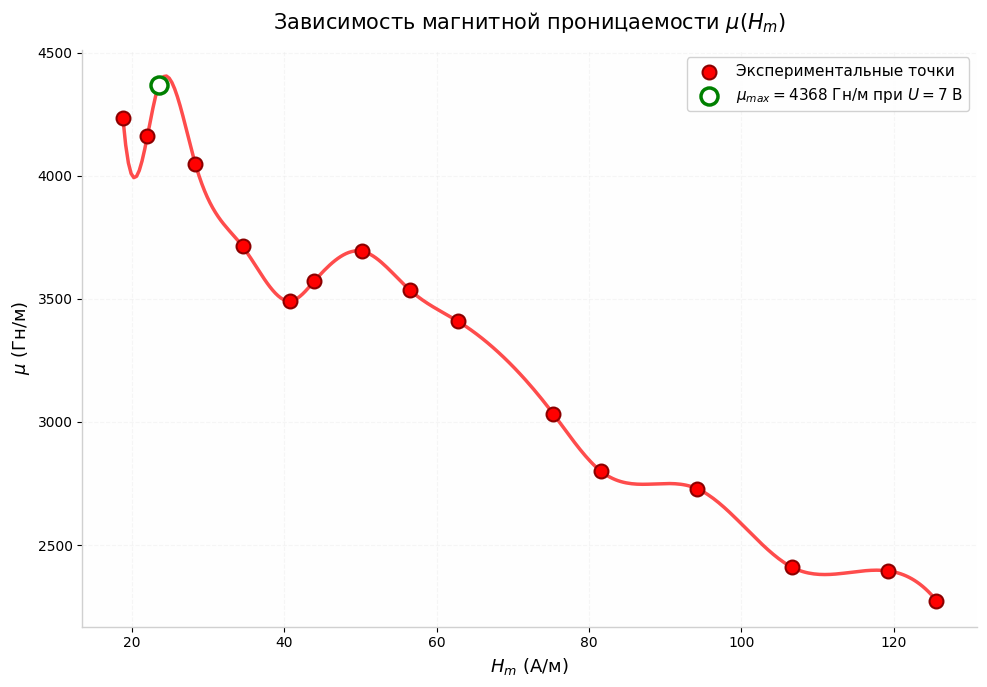
\includegraphics[width=0.5\linewidth]{pic/image (1).png}
    \caption{Зависимость магнитной проницаемости $\mu(H_m)$}
    \label{fig:placeholder}
\end{figure}

\begin{figure}[!h]
    \centering
    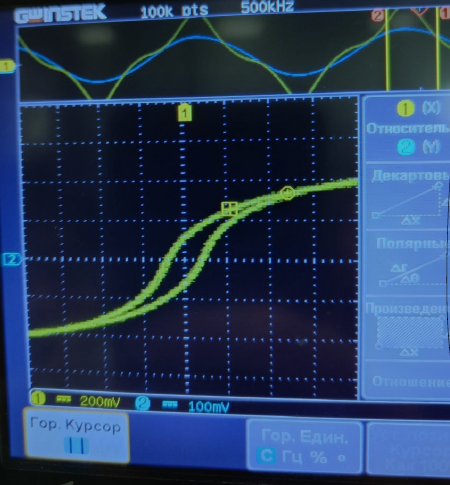
\includegraphics[width=0.38\linewidth]{pic/sp20260417_004034_310.png}
    \caption{Петля гистерезиса}
    \label{fig:placeholder}
\end{figure}

\newpage

\section{Вывод}

В ходе выполнения лабораторной работы изучены свойства ферромагнетика (сердечника трансформатора):

\begin{enumerate}
    \item Получена зависимость магнитной индукции от напряженности поля $B = B(H)$ -- кривая начального намагничивания (по вершинам частных петель гистерезиса).
    
    \item По предельной петле гистерезиса определены основные характеристики материала:
    \begin{itemize}
        \item Коэрцитивная сила $H_c = 12{,}6$~А/м
        \item Остаточная индукция $B_r = 0{,}108$~Тл
        \item Индукция насыщения $B_m = 0{,}359$~Тл (при $H_m = 125{,}6$~А/м)
        \item Начальная магнитная проницаемость $\mu_m = 2274$~Гн/м
    \end{itemize}
    
    \item Получена зависимость магнитной проницаемости от напряженности поля $\mu = \mu(H)$. 
    Установлено, что максимальная проницаемость $\mu_{\max} = 4368$~Гн/м 
    достигается при $H = 23{,}5$~А/м ($U = 7$~В), что соответствует наиболее крутому участку кривой намагничивания.
    
    \item Рассчитана мощность потерь энергии на перемагничивание при частоте $f = 20$~Гц 
    и площади петли гистерезиса $S_{\text{пг}} = 8$~клеток: 
    $P = (4{,}5 \pm 0{,}9)$~мВт (погрешность $\sim 20\%$).
\end{enumerate}

Построенные графики $B_m(H_m)$ и $\mu(H_m)$ демонстрируют характерное поведение 
ферромагнитного материала: нелинейный рост индукции с увеличением поля с последующим 
насыщением и наличие выраженного максимума магнитной проницаемости в области 
средних значений напряженности магнитного поля.